\documentclass[10pt]{article}\usepackage[margin=.65in]{geometry}\usepackage[T1]{fontenc}\usepackage{graphicx}\setlength{\parindent}{0pt}\setlength{\parskip}{7pt}\sloppy\begin{document}{\large Native signed collector: ordered capture and prefix checks}\par Software source extension at parent f7cb04ca67. Final control receipt: check-pwKutLmL; existing native regression: native-check-5eSIvdq6. This record covers one fixed known-answer target, six configurations and bounded deterministic software checks. The graph shows event counts, not timings or cost ratios.\par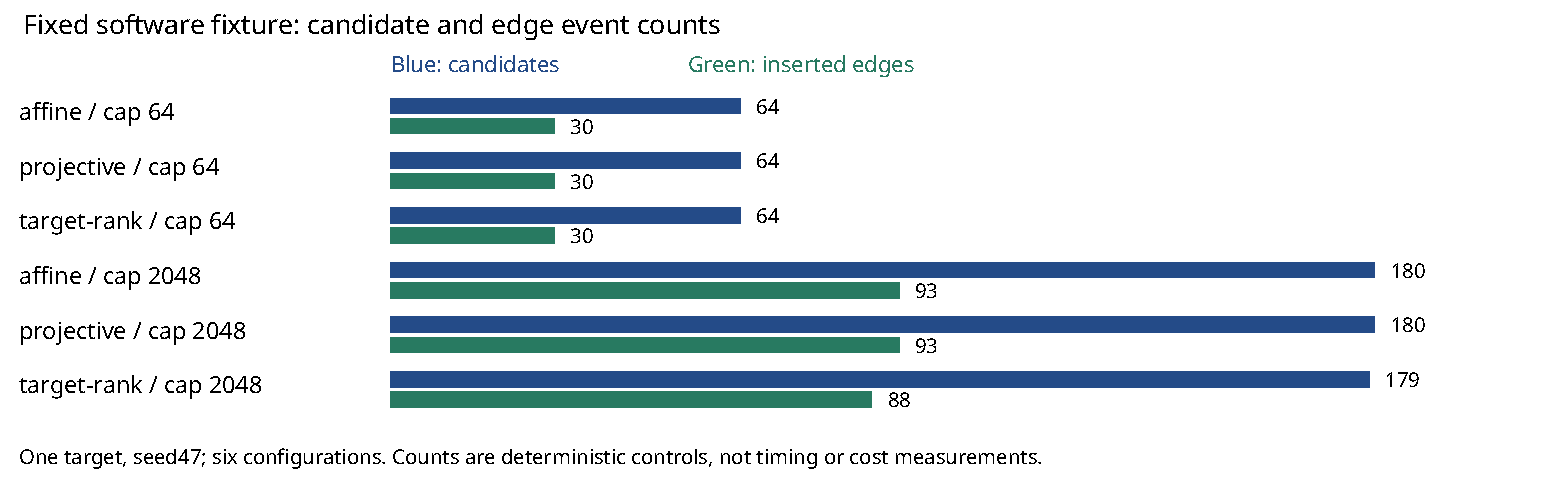
\includegraphics[width=\linewidth]{diagram.pdf}\par Implemented. An optional fallible observer now runs at actual two-choice collector call sites. It records candidates before selection, new nodes, exact submitted signed edges and native returns, plus duplicate, identity, nonsplit, restart and terminal dispositions. Existing entry points select the absent observer. The separate in-memory recorder enforces record/serialized-byte limits and rejects continuation after terminal or failure.

Checked outputs. Three capture-control tests and all six existing follow-up tests passed. Every complete observed result, including recorded arithmetic counters, equals the corresponding unobserved result. Six configurations on the fixed p=739 target (target=2G, source r=34147, generator seed 23, walk seed 47) contributed 364 captured edge prefixes. Full source/transfer coordinates and parameters are in controls.json. These configurations are not independent target samples; no uncertainty estimate or extrapolation is made.

Prefix algebra. Each captured edge was replayed through a fresh native SignedGraph. A separate offline linear-information implementation checked consistency and whether the target is uniquely determined at every prefix. It used [A,-b,-a], excluded node 0 and zero-extended older rows as nodes appeared. Three 64-candidate controls each had 30 edge prefixes and no scalar return. At the 2048 cap, affine/projective modes returned scalar 2 after 180 candidates/93 edges; target-rank mode returned scalar 2 after 179 candidates/88 edges. Every returned scalar was checked in the source group.

Coverage limits. Duplicate, identity and restart events were absent from these controls; their hooks need dedicated coverage. The rank preview is retained as a source-local score and is not assumed identical to global target information. The observer performs no online rank analysis. Serialization and allocation are unpriced, so this packet supplies no new matched-cost comparison. Recorder bounds are serialized-output bounds, not whole-process memory bounds.

Failures and reviews. The first assumed p=19 fixture returned None and two tests failed; the existing p=739 fixture replaced it, with the failed attempt retained. The original native manifest lacked Cargo.lock and its locked test invocation failed before compilation. A scoped locked manifest now points at the same original lib.rs and runs its six follow-up tests. Independent source review remains pending because delegated reviewers are unavailable. The earlier full-root library build failures remain in the preceding target-stream-implementation packet.

Sources and next joins. The inspected source contract is ../packets/target-stream-reconciliation/SOURCE-MAP.md; native behavior is in src/cryptanalysis/three\_leads\_followup.rs and SignedGraph in three\_leads.rs. The rank criterion is implemented in ../../five-followups/rank-information. Exact dependency hashes are retained with final checks. Next: exceptional-disposition controls, authenticated durable stream publication and a strict offline loader, independent review, and Kummer-specific integration. The full 1,260-target and complete-cost obligations retain their existing admission and budget gates.
\end{document}